\documentclass[12pt]{extarticle} % Note the extarticle document class
\usepackage{graphicx} % Required for inserting images
\usepackage{geometry}
 \geometry{a4paper, portrait, margin=1in}
\usepackage{amsmath}

\usepackage[
backend=biber,
style=numeric,
sorting=none
]{biblatex}
\addbibresource{bibliography.bib}

\usepackage[colorlinks=true,linkcolor=blue,citecolor=blue,urlcolor=blue]{hyperref}

\usepackage{newunicodechar}
\newunicodechar{−}{-}

\author{\textbf{Proposer}: Thach Dang \\ \textbf{Mentor}: Stephen Padin (Research Professor)}
\title{Radio Holography for the Deep Synoptic Array}
\date{} % clear date

\begin{document}

\maketitle

\section{Summary}
The objective of this project is to apply holography to quantify the surface accuracy of Deep Synoptic Array antennas by using signals from bright astronomical objects. This is a crucial measurement because it would provide a means for verification that the antennas are aligned and working as expected.

\section{Introduction}
\subsection{Radio Astronomy}
Radio waves hold a unique place in astronomy due to Earth’s atmosphere, which is highly transparent to optical and radio wavelengths in the meter to centimeter range, while absorbing ultraviolet, X-rays, gamma rays, much of the infrared, and very long-wavelength radio emission. This transparency allows large ground-based radio telescopes to operate without space deployment. The field expanded rapidly with the discovery of the 21\,cm hydrogen line in the mid-20th century. The observations in the radio part of the spectrum are crucial for the study of neutral hydrogen, cold molecular gas, and synchrotron radiation. \cite{radioastro}.

\subsection{The Deep Synoptic Array}
\noindent The Deep Synoptic Array, or DSA, is a radio telescope array under construction in Spring Valley, Nevada - consists of 1650 6\,m diameter dishes with a broad frequency range of 0.7–2.0 GHz, capable of detecting over one billion unique radio sources across the northern sky \cite{DSA}\cite{DSAScience}. The instrument's scientific focus is split into four pillars: multi-messenger astronomy, our cosmic history, the dynamic radio sky, and the dark sector. This mission will collectively address 20 of the 24 priority questions identified in the Astro2020 Decadal Survey \cite{DSAScience}. Although the plan for DSA is to be in Nevada, its prototypes, as seen in figure \ref{fig:DSALocation}, are currently at the Owens Valley Radio Observatory (OVRO) for testing. The proposer will  use this array to test holography techniques for DSA.
\begin{figure}[h]
    \centering
    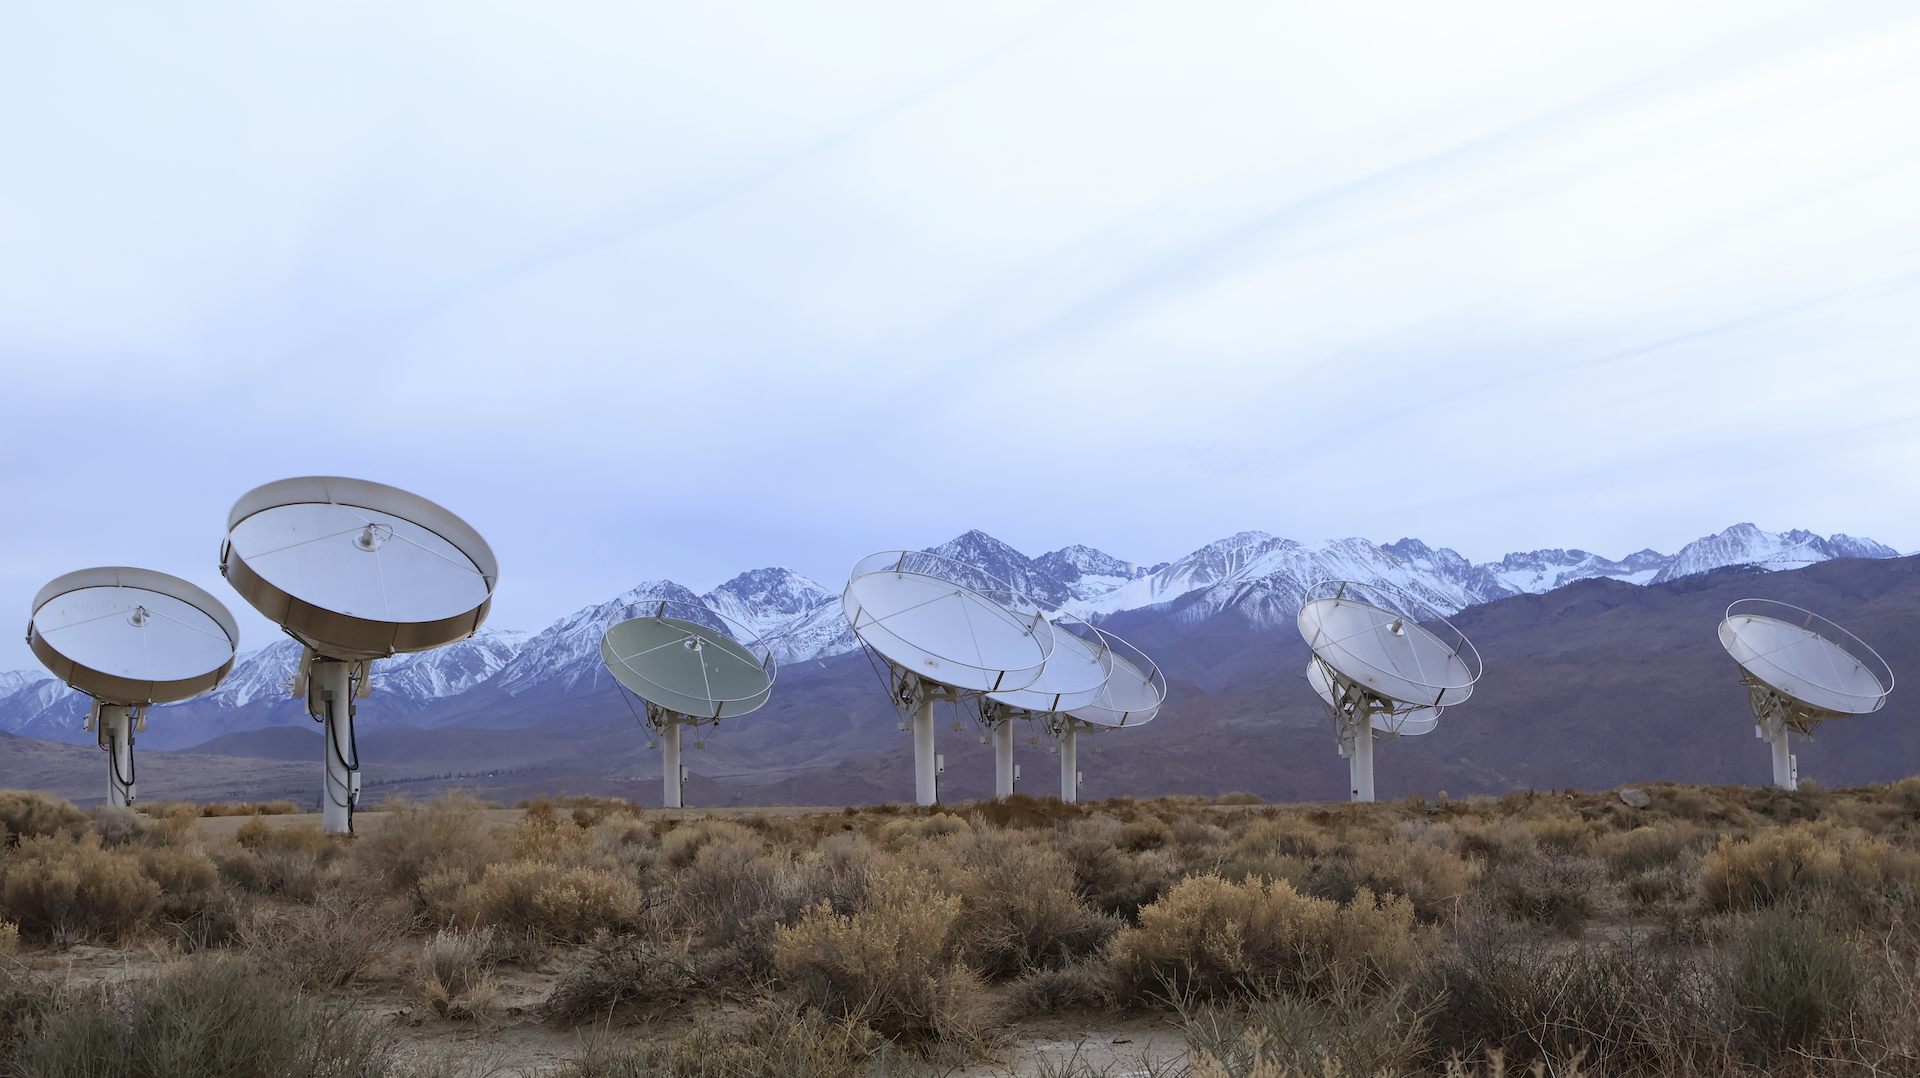
\includegraphics[width=1\linewidth]{images/TestArraySmall.png}
    \caption{DSA test array at OVRO}
    \label{fig:DSALocation}
\end{figure}
\newpage
\subsection{Radio Holography}
Surface irregularities on a radio antenna can significantly spoil its angular response, impacting the antenna's ability perform high quality observations. This is why it is important to measure and understand an antenna's surface. A method to do this is radio holography developed by P.F. Scott and M. Ryle \cite{PF_scott}. Holography is performed by using either a celestial or man made source to measure the antenna's reception pattern in amplitude and phase across an angular grid. This is used to create a contour map of the reflector surface. \\

\noindent The steps to perform holography can be simplified into:

\begin{enumerate}
    \item Identify a stable signal source which can either be a celestial object such as a star or a man-made transmitter on a high tower. 
    \item Set up an interferometric baseline between two antennas connected to a complex correlator, which multiplies the voltage between the two antennas. One of the antennas, the reference antenna is pointed at the source on boresight during the measurement to provide a stable phase reference, while the other antenna is used to measure the reception pattern.
    \item Direct the test antenna to a succession of points $(\theta, \phi)$ away from the source. This measures the reception pattern (the diffraction pattern) of the antenna in both amplitude and phase across a grid
    \item Fourier transform to convert the measured reception pattern into a map of the aperture illumination. An example is shown in figure \ref{fig:surface}. 
    \item Calculate the uncertainty of the surface error $\delta \epsilon$
\end{enumerate}

\begin{figure}[h]
    \centering
    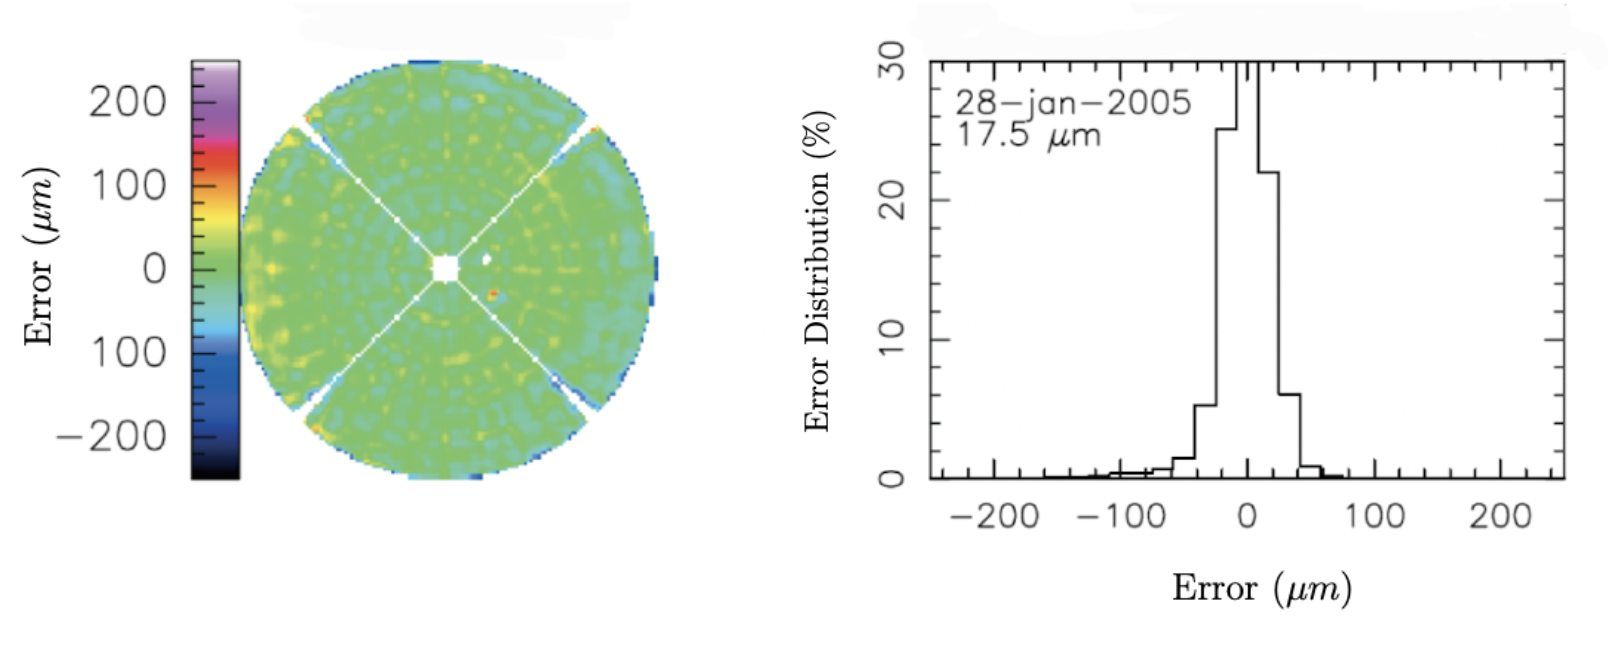
\includegraphics[width=1\linewidth]{images/Surface Map and Distribution.png}
    \caption{\textit{Left:} Surface error map of an Atacama Large Millimeter/submillimeter Array antenna by the ALCATEL EIE Consortium. \textit{Right:} Distribution of surface error on AEC antenna $\epsilon$  \cite{Mangum_2006}}
    \label{fig:surface}
\end{figure}

\section{Objectives and Approach}\label{sec:Objectives}
Implementing holography on DSA antennas presents several technical challenges, which are outlined and addressed below:
\begin{enumerate}
    \item \textbf{Low sensitivity and SNR limitations:} Small DSA antennas have low signal-to-noise ratios due to the relation $SNR \propto \sqrt{A_1 A_2}$ where $A_1$ and $A_2$ are the areas of the antennas in the interferometer. This leads to noisy correlator outputs and surface maps since $\delta \epsilon \propto \frac{1}{SNR}$. This can be mitigated by pairing a 6\,m test antenna with a larger 10\,m or 40\,m reference antenna (since $SNR \propto \sqrt{A_1 A_2} \propto d_1 d_2$) and observing very bright celestial sources above 100\,Jy such as Cass A, Cygnus A, Tau A, Virgo A, or Herc A to increase signal strength and improve surface accuracy \cite{HoloMeasurementsDSA}.
    \item \textbf{Radio Frequency Interference (RFI):} Modern communication systems such as cell phones and satellite communication systems introduce RFI that degrades measurement quality. This can be addressed by collecting test data to characterize interference and applying RFI filters if needed.
    \item \textbf{Geometric and mechanical phase errors:} Non-intersecting azimuth, elevation, and optical axes cause phase delays ($\Delta d$) depending on pointing offsets that must be modeled correctly. In the analysis pipeline, mechanical axis offsets must be accounted for and we must use exact trigonometric expressions because the response is mapped over large angles.
\end{enumerate}
% \section{Approach}
% \noindent Performing holographic measurements on the DSA prototype antenna requires addressing technical challenges mentioned in section \ref{sec:Objectives}. Below are how the proposer will address these challenges:  

% \begin{itemize}
%     \item Challenges relating to the small diameter of the DSA antenna can be dealt with by making modifications to modeling and data analysis pipelines
%     \begin{itemize}
%         % \item Using exact geometric modeling with exact trigonometric closed-form expressions to maintain exact surface mapping over large angular ranges.
%         \item Account for mechanical axis offsets to adjust for exact separations among non-intersecting azimuth, elevation, and optical axes to compute the additional phase delay ($\Delta d$), thereby avoiding incorrect assignment of mechanical path length changes to surface mapping.
%     \end{itemize}
%     \item RFI can be addressed by taking test data to characterize interference, then apply RFI filters if needed.
%     \item The problem due to sensitivity and low SNR can be solved by increasing signal strength from
%     \begin{itemize}
%         \item  Employing a large 10m reference antenna with the 6m test antenna to observe extremely bright celestial sources to increase the $SNR$, since $SNR\propto \sqrt{A_1 A_2} \propto \sqrt{\pi\frac{d^2}{4}}\propto d$, thereby also achieving a more accurate reflector surface profile. 
%         \item Observing a bright celestial source $> 100$ Jy such as Cass A, Cygnus A, Tau A, Virgo A, or Herc A \cite{HoloDSAConsiderqations}
%     \end{itemize}
 
% \end{itemize}

\section{Work Plan}
Week 1: Learn about holography data analysis.\\
Week 2: Write code to simulate a measurement and analyze the simulated data\\
Week 3: Learn how to drive DSA antennas and how to get data out of the correlator \\
Week 4: Go to OVRO to set up the reference antenna electronics (on a DSA antenna or an old OVRO 10m antenna)\\
Week 5: Write interim report\\
Week 6: Take some test data, and add RFI filters if needed\\
Week 7: Run a holography measurement\\
Week 8: Analyze the data from the previous week's holography measurement\\
Week 9: Figure out any problem, fix it, then repeat the measurement and analysis\\
Week 10: Document the process and write final report\\

\printbibliography[heading=bibintoc,title={References}] 

\end{document}
